\documentclass[a4j,10pt,titlepage]{jsarticle}
\renewcommand{\headfont}{\bfseries}
\usepackage[dvipdfmx]{graphicx}
\usepackage{url}
\usepackage{here}
\title{情報科学演習C レポート1}
\author{藤田 勇樹 \\
大阪大学 基礎工学部 情報科学科 ソフトウェア科学コース\\
学籍番号: 09B16068 \\
メールアドレス: u461566g@ecs.osaka-u.ac.jp \\
担当教員\\
小島 英春 助教授 \\
内山 彰 助教授}
\date{提出日: 2018年4月22日}

\begin{document}
\maketitle
\section{課題1-1}
\subsection{pingコマンド}\label{sec:ping}
\verb|ping|コマンドを実行すると,以下のような出力が得られる.
\begin{verbatim}
$ ping exp101 
PING exp101.exp.ics.es.osaka-u.ac.jp (192.168.16.65) 56(84) bytes of data.
64 bytes from exp101.exp.ics.es.osaka-u.ac.jp (192.168.16.65): icmp_seq=1 ttl=64 time=0.134 ms
64 bytes from exp101.exp.ics.es.osaka-u.ac.jp (192.168.16.65): icmp_seq=2 ttl=64 time=0.180 ms
64 bytes from exp101.exp.ics.es.osaka-u.ac.jp (192.168.16.65): icmp_seq=3 ttl=64 time=0.194 ms
64 bytes from exp101.exp.ics.es.osaka-u.ac.jp (192.168.16.65): icmp_seq=4 ttl=64 time=0.209 ms
64 bytes from exp101.exp.ics.es.osaka-u.ac.jp (192.168.16.65): icmp_seq=5 ttl=64 time=0.185 ms

--- exp101.exp.ics.es.osaka-u.ac.jp ping statistics ---
5 packets transmitted, 5 received, 0% packet loss, time 3999ms
rtt min/avg/max/mdev = 0.134/0.180/0.209/0.027 ms
\end{verbatim}

オンラインマニュアルで\verb|ping|について調べたところ,以下の事柄がわかった.\verb|ping|コマンドでは,引数に指定されたホストにICMPプロトコルのECHO\_REQUESTを送り,それが正しく送られたか,またそれにかかった時間を出力する.ICMPプロトコルとは,マシンの状態やエラーメッセージなどを送受信するプロトコルで,ECHO\_REQUESTはICMPでやりとりするメッセージの一種である.

実際の出力の意味を説明する.
\begin{verbatim}
64 bytes from exp101.exp.ics.es.osaka-u.ac.jp (192.168.16.65): icmp_seq=1 ttl=64 time=0.134 ms
\end{verbatim}
これは,64バイトのパケット1個目をexp101(IPアドレス192.168.16.65)にTTL=64で送り,応答を受け取るまで0.134ミリ秒かかったということである.TTLとはTime to Liveの略で,パケットがあるノードから別のノードに受け渡される回数の上限を表す.パケットがノードから送信されるたびにTTLは1ずつ減り,0になるとそのパケットは宛先に辿りつけなかったものとして破棄される.

しかし,yahoo.comなどの外部ホストに\verb|ping|を実行したところパケットが届かなかった.これについては\ref{sec:traceroute}で考察する.

\subsection{ドメイン名とIPアドレス}\label{sec:domainip}
\url{http://www-higashi.ist.osaka-u.ac.jp/}と\url{http://133.1.17.66/}にアクセスしたところ,全く同じページが表示された.そのため,\verb|www-higashi.ist.osaka-u.ac.jp|と\verb|133.1.17.66|は同じものを表すと思われる.

\subsection{nslookupコマンド}\label{sec:nslookup}
nslookupをmanコマンドで調べたところ,nslookupはホスト名に対応するIPアドレスを調べるコマンドであった.実際に,\verb|www-higashi.ist.osaka-u.ac.jp|を実行すると,\ref{sec:domainip}節の通り\verb|133.1.17.66|が得られた.また土屋研\url{www-ise4.ist.osaka-u.ac.jp}に対応するのは\verb|133.1.16.2|であった.



\section{課題1-2}
\subsection{arpコマンド}
ARPは,IPアドレスがわかっているホストにMACアドレスを問い合わせるプロトコルである.また,ARPテーブルとは,過去の通信でARPプロトコルを使用した際に得られたIPアドレスとMACアドレスの対応をキャッシュとして保存したものである.
\verb|arp|コマンドではARPテーブルを表示する.実際に\verb|arp -a|コマンドを実行すると以下のような出力が得られる.
\begin{verbatim}
exp029.exp.ics.es.osaka-u.ac.jp (192.168.16.62) at 00:50:56:b7:0d:47 [ether] on ens192
cups.exp.ics.es.osaka-u.ac.jp (192.168.16.253) at 00:50:56:b7:5b:4b [ether] on ens192
exp036.exp.ics.es.osaka-u.ac.jp (192.168.16.52) at 00:50:56:b7:59:b6 [ether] on ens192
? (192.168.16.254) at 14:18:77:10:31:aa [ether] on ens192
dhcp-01.exp.ics.es.osaka-u.ac.jp (192.168.16.240) at 00:50:56:b7:21:6e [ether] on ens192
svm-01.exp.ics.es.osaka-u.ac.jp (192.168.16.241) at 02:a0:98:c4:b2:cf [ether] on ens192
\end{verbatim}
exp029の端末で\verb|ifconfig|でMACアドレスを確認してもらうと,確かに同じMACアドレスであった.

\subsection{ping後のarpコマンド}
\verb|ping exp092|を行った後に再びarpコマンドを実行すると,以下の行が追加されていた.
\begin{verbatim}
exp092.exp.ics.es.osaka-u.ac.jp (192.168.16.18) at 00:50:56:b7:79:90 [ether] on ens192
\end{verbatim}
このことから,ARPテーブルには過去の通信で得られたIPアドレスとMACアドレスの対応が自動で格納されることがわかる.

\subsection{tracerouteコマンド}\label{sec:traceroute}
www.ics.es.osaka-u.ac.jpとicsintgw.ics.es.osaka-u.ac.jpにそれぞれ\verb|traceroute|を実行すると,どちらも以下のような出力が得られた.
\begin{verbatim}
traceroute to icsintgw.ics.es.osaka-u.ac.jp (133.1.240.81), 30 hops max, 60 byte packets
 1  192.168.16.254 (192.168.16.254)  0.375 ms  0.446 ms  0.508 ms
 2  icsintsvgw.ics.es.osaka-u.ac.jp (133.1.240.254)  0.720 ms  0.882 ms  1.006 ms
 3  icsintgw.ics.es.osaka-u.ac.jp (133.1.240.81)  1.777 ms  2.392 ms  9.386 ms
\end{verbatim}

ただし,icsintgw.ics.es.osaka-u.ac.jpは終了したが,www.ics.es.osaka-u.ac.jpはicsintgw.ics.es.osaka-u.ac.jpまで辿った後,応答がないことを表す``* * *''が表示され続けた.

演習室の環境ではhttp/httpsでしか外部と通信できないが,\verb|traceroute|ではオンラインマニュアルによるとICMPを使用しているため,ゲートウェイicsintgw.ics.es.osaka-u.ac.jpで通信が止められているものと考えられる.
\ref{sec:ping}節でyahoo.comなどの適当なドメインへの\verb|ping|が届かなかったのも同様の理由のためであると思われる.

\subsection{演習室のネットワーク構成}
前節までの結果より,演習室のネットワーク構成は以下の図\ref{fig:netstat}のようになっていると思われる.
\begin{figure}[H]
\centering
 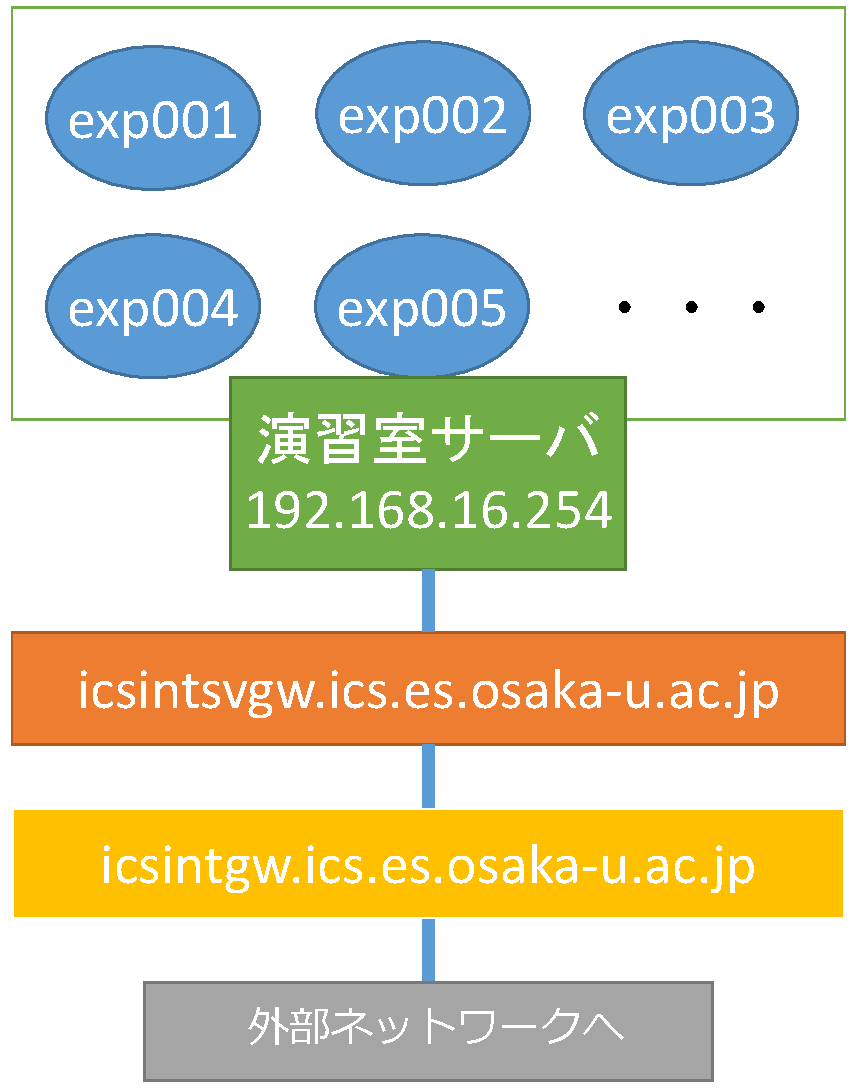
\includegraphics[scale=0.5]{netstat_cropped.pdf}
 \caption{演習室のネットワーク構成の予想}
 \label{fig:netstat}
\end{figure}

\subsection{netstatコマンド}
\verb|netstat -r|を実行すると,以下のような出力が得られた.
\begin{verbatim}
$ netstat -r
カーネルIP経路テーブル
受信先サイト    ゲートウェイ    ネットマスク   フラグ   MSS Window  irtt インタフェース
default         192.168.16.254  0.0.0.0         UG        0 0          0 ens192
link-local      *               255.255.0.0     U         0 0          0 ens192
192.168.16.0    *               255.255.255.0   U         0 0          0 ens192
\end{verbatim}

オンラインマニュアルによると,\verb|netstat -r|コマンドでは,カーネルのルーティングテーブルを出力する.ルーティングテーブルとは,受け取ったパケットの宛先に応じて,次にどのノードにパケットを転送すればよいかを記録してあるものである.例えば,受け取ったパケットの宛先が133.1.17.66であれば,一番上の192.168.16.254に転送する.

\subsection{再びarpコマンド}
前節までの作業を行った次の週に\verb|arp -a|コマンドを実行すると,演習室の端末のARPテーブルが消えていた.このことから,自動的に追加され長時間使用していないARPテーブルは削除されることがわかる.

\section{課題1-3}
\subsection{標準ライブラリ関数とシステムコールの違い}
C言語の標準ライブラリ関数とシステムコールの違いについて述べる.課題での例では,fwrite()とwrite()はともにファイルへの書き込みを行う関数であるが,fwrite()はどの環境でも使用できる一方,write()はPOSIX環境でのみ使用でき,Windowsなどでは使用できない.ただし,標準ライブラリ関数は環境に依存しない方法であるが,その実装にはシステムコールが使用されているため,生のシステムコールに比べてオーバーヘッドが生じる場合がある.

\subsection{straceコマンド}
\begin{verbatim}
$ strace -c echo hello
\end{verbatim}
を実行したところ,以下の出力が得られた.

\begin{verbatim}
% time     seconds  usecs/call     calls    errors syscall
------ ----------- ----------- --------- --------- ----------------
  0.00    0.000000           0         1           read
  0.00    0.000000           0         1           write
  0.00    0.000000           0         3           open
  0.00    0.000000           0         5           close
  0.00    0.000000           0         4           fstat
  0.00    0.000000           0         8           mmap
  0.00    0.000000           0         4           mprotect
  0.00    0.000000           0         1           munmap
  0.00    0.000000           0         3           brk
  0.00    0.000000           0         3         3 access
  0.00    0.000000           0         1           execve
  0.00    0.000000           0         1           arch_prctl
------ ----------- ----------- --------- --------- ----------------
100.00    0.000000                    35         3 total
\end{verbatim}

ここでは,``\verb|echo hello|''を実行し,どのシステムコールが何回呼ばれたかをcallsの列に出力している.また,それぞれのシステムコールの種類ごとにかかった時間とその割合も出力される.

また,``\verb|ls|''では以下の出力が得られた.出力されるcallsの数はディレクトリによって異なる場合がある.
\begin{verbatim}
% time     seconds  usecs/call     calls    errors syscall
------ ----------- ----------- --------- --------- ----------------
  0.00    0.000000           0         7           read
  0.00    0.000000           0         5           write
  0.00    0.000000           0         9           open
  0.00    0.000000           0        11           close
  0.00    0.000000           0        10           fstat
  0.00    0.000000           0        19           mmap
  0.00    0.000000           0        12           mprotect
  0.00    0.000000           0         1           munmap
  0.00    0.000000           0         3           brk
  0.00    0.000000           0         2           rt_sigaction
  0.00    0.000000           0         1           rt_sigprocmask
  0.00    0.000000           0         2           ioctl
  0.00    0.000000           0         7         7 access
  0.00    0.000000           0         1           execve
  0.00    0.000000           0         2           getdents
  0.00    0.000000           0         1           getrlimit
  0.00    0.000000           0         2         2 statfs
  0.00    0.000000           0         1           arch_prctl
  0.00    0.000000           0         1           set_tid_address
  0.00    0.000000           0         1           set_robust_list
------ ----------- ----------- --------- --------- ----------------
100.00    0.000000                    98         9 total
\end{verbatim}

\verb|echo hello|に比べ,いくつかのシステムコールが追加されているほか,open,closeなどファイル操作の回数が増えている.しかし,``\verb|ls|''コマンドはファイルの内容を調べるものではないため,他の要因でopenやcloseの回数が増えていると考えた.そこで,openで何を開いているかを調べるため以下のコマンドを実行した.

\begin{verbatim}
strace ls 2>&1 1>/dev/null | grep open
\end{verbatim}

オプションなしの\verb|strace|コマンドは呼び出されたシステムコールを逐一出力する.また,\verb|strace|コマンドの出力は調べる対象のコマンドの出力と被らないようにするためか標準エラー出力に出力されている.そのため標準エラー出力のみから``open''のある行を取り出している.このコマンドを実行すると,以下の出力が得られた.

\begin{verbatim}
open("/etc/ld.so.cache", O_RDONLY|O_CLOEXEC) = 3
open("/lib/x86_64-linux-gnu/libselinux.so.1", O_RDONLY|O_CLOEXEC) = 3
open("/lib/x86_64-linux-gnu/libc.so.6", O_RDONLY|O_CLOEXEC) = 3
open("/lib/x86_64-linux-gnu/libpcre.so.3", O_RDONLY|O_CLOEXEC) = 3
open("/lib/x86_64-linux-gnu/libdl.so.2", O_RDONLY|O_CLOEXEC) = 3
open("/lib/x86_64-linux-gnu/libpthread.so.0", O_RDONLY|O_CLOEXEC) = 3
open("/proc/filesystems", O_RDONLY)     = 3
open("/usr/lib/locale/locale-archive", O_RDONLY|O_CLOEXEC) = 3
open(".", O_RDONLY|O_NONBLOCK|O_DIRECTORY|O_CLOEXEC) = 3
\end{verbatim}

ここで,libc.so.6などの/lib配下のファイルは,標準ライブラリ関数の実装であり,普段C言語で標準ライブラリを使用した際には,実際にはこれらのファイルの内容が実行される.
比較のため,``\verb|echo hello|''でも同様の調査を行った.

\begin{verbatim}
open("/etc/ld.so.cache", O_RDONLY|O_CLOEXEC) = 3
open("/lib/x86_64-linux-gnu/libc.so.6", O_RDONLY|O_CLOEXEC) = 3
open("/usr/lib/locale/locale-archive", O_RDONLY|O_CLOEXEC) = 3
\end{verbatim}

これらを比較すると,\verb|ls|の方では使用しているライブラリが増えているほか,/proc/filesystemsなどファイルシステム関連の情報を参照していることがわかる.また,カレントディレクトリを開くのにもopenを使用している.

また,``\verb|ping exp001|''では以下の出力が得られた.

\begin{verbatim}
ping: icmp open socket: Operation not permitted
% time     seconds  usecs/call     calls    errors syscall
------ ----------- ----------- --------- --------- ----------------
  0.00    0.000000           0        16           read
  0.00    0.000000           0         1           write
  0.00    0.000000           0        15           open
  0.00    0.000000           0        20           close
  0.00    0.000000           0         2           stat
  0.00    0.000000           0        15           fstat
  0.00    0.000000           0         2           poll
  0.00    0.000000           0        23           mmap
  0.00    0.000000           0        14           mprotect
  0.00    0.000000           0         4           munmap
  0.00    0.000000           0         3           brk
  0.00    0.000000           0         1           ioctl
  0.00    0.000000           0         9         9 access
  0.00    0.000000           0         1           dup
  0.00    0.000000           0         1           getpid
  0.00    0.000000           0         5         1 socket
  0.00    0.000000           0         4         2 connect
  0.00    0.000000           0         1           sendto
  0.00    0.000000           0         1           recvfrom
  0.00    0.000000           0         1           getsockname
  0.00    0.000000           0         1           execve
  0.00    0.000000           0         4           fcntl
  0.00    0.000000           0         2           getuid
  0.00    0.000000           0         1           setuid
  0.00    0.000000           0         1           geteuid
  0.00    0.000000           0         7           capget
  0.00    0.000000           0         1           capset
  0.00    0.000000           0         2           prctl
  0.00    0.000000           0         1           arch_prctl
------ ----------- ----------- --------- --------- ----------------
100.00    0.000000                   159        12 total
\end{verbatim}

\verb|echo|の出力に比べ,socket(2)やconnect(2)などのネットワーク関連のシステムコールが加わっていることがわかる.

\section{発展課題}
\subsection{ネットワーク関連のコマンド}
\subsubsection{telnet}
\verb|telnet|コマンドは,他のマシンの遠隔操作を行うためのコマンドである.引数に指定したIPアドレスのマシンに接続する.
\verb|telnet 127.0.0.1|を実行しパスワードを入力するとWelcome to Ubuntu 16.04.4 LTS ... 等のメッセージが表示された後,通常通りの端末操作が可能となった.
また友人のマシンにアクセスしパスワードを入力してもらうと,同様にそのマシンに対しての端末操作が可能となった.

\subsubsection{rsh}
\verb|rsh|コマンドは,他のマシンに接続し引数に指定したコマンドを実行するコマンドである.\verb|rsh exp029 ls|を実行しパスワードを入力してもらうと,exp029のホームディレクトリの内容が出力された.

\subsubsection{ftp}
\verb|ftp|コマンドは,FTPサーバに接続しファイルのやり取りをするコマンドである.引数か起動後にopenコマンドでFTPサーバのアドレスを指定して接続する.しかしFTPサーバの所在が不明だったため使用できなかった.

\verb|finger|コマンドおよび\verb|talk|コマンドは演習室の環境ではインストールされていないため使用できずマニュアルも表示できなかった.

\subsection{hello100回}
以下のプログラムを,コメントアウトを切り替えて実行し,\verb|strace -c|を用いてシステムコールの呼び出し回数を比較する.
\begin{verbatim}
#include <stdio.h>
#include <string.h>
#include <unistd.h>
#define COUNT 100
int main(int ac, char* av[]){
    int i;
        // [下記 2 行の内、いずれかをコメントアウトする]
        char message[] = "hello";
        // char message[] = "hello\n";
    for(i = 0; i < COUNT; i ++){
        // [下記 2 行の内、いずれかをコメントアウトする]
        fwrite(message, strlen(message), 1, stdout);
        // write(0, message, strlen(message));
    }
    return 0;
}
\end{verbatim}

以下の表\ref{table:strace}にそれぞれのプログラムでの\verb|strace|の出力を述べる.ただし,ここではシステムコールの回数であるcallsの部分のみ載せる.

\begin{table}[H]
  \begin{center}
  \caption{straceの出力}
  \label{table:strace}
  \begin{tabular}{l|c|c|c|c}\hline
  syscall & 改行なし,fwrite & 改行なし,write & 改行あり,fwrite & 改行あり,write \\ \hline \hline
read & 1 & 1 & 1 & 1 \\ \hline
write & 1 & 100 & 100 & 100 \\ \hline
open & 2 & 2 & 2 & 2 \\ \hline
close & 2 & 2 & 2 & 2 \\ \hline
fstat & 3 & 2 & 3 & 2 \\ \hline
mmap & 7 & 7 & 7 & 7 \\ \hline
mprotect & 4 & 4 & 4 & 4 \\ \hline
munmap & 1 & 1 & 1 & 1 \\ \hline
brk & 3 & 1 & 3 & 1 \\ \hline
access & 3 & 3 & 3 & 3 \\ \hline
execve & 1 & 1 & 1 & 1 \\ \hline
arch\_prctl & 1 & 1 & 1 & 1 \\ \hline
  \end{tabular}
  \end{center}
\end{table}

注目すべきは,改行なし,fwriteでのみwriteが1回しか呼ばれていない点である.改行あり,fwriteではwriteが100回呼ばれていることを踏まえると,fwriteでは改行を出力文字として受け取るまでは出力する文字はバッファリングしておき,改行を受け取るかファイルストリームが閉じられる時に出力すると考えられる.

詳しく調べてみると,このバッファリングの方針はsetvbuf()関数で変更できることがわかった.そこで,この関数を追加し\_IONBF(バッファリングを一切しない)を設定すると,改行なし,fwriteでもwriteが100回呼び出されるようになった.

この他の違い(fstatとbrkの数)はどちらもfwriteとwriteのどちらを使うかで異なっているので,fwriteの処理の一環として呼び出されていると思われる.
\end{document}
